\documentclass{scrbook}
\usepackage{graphicx} % Required for inserting images
\usepackage{tabularx} % Required for fixed width tables
\usepackage{scrlayer-scrpage} % Required for the subtitles
\usepackage{url} % Required for the URLs
\usepackage{hyperref} % Required for the URLs
\usepackage{listings} % Required for the code snippets
\usepackage{mathtools} % Required for the system of equations
\usepackage{amsmath,amssymb} % Required for some math symbols
\usepackage{enumitem} % Required for lettered lists

% Put the caption of the snippets at the bottom and allow math symbols usage
\lstset{
    captionpos=b,
    mathescape=true,
    escapeinside={(*@}{@*)}
}

% Required for circled numbers
\usepackage{tikz}
\newcommand*\circled[1]{\tikz[baseline=(char.base)]{
            \node[shape=circle,draw,inner sep=2pt] (char) {#1};}}


\title{Solidity hands-on lesson}
\subtitle{Ambient intelligence course (A.Y. 2025/2026)\\Topic taught by Prof. Arnaldo Tomasino}
\author{Gabriele Colapinto}
\date{\today}

\begin{document}

\maketitle
\thispagestyle{empty}

{\Large\textbf{License}} \\
{Notes from Ambient intelligence (A.Y. 2025/2026) by Gabriele Colapinto. 
Course taught by professors Michele Ruta, Floriano Scioscia, Arnaldo Tomasino, Davide Loconte — 
Licensed under CC BY-NC 4.0.\\
\url{https://creativecommons.org/licenses/by-nc/4.0/}}

\vspace*{\fill}
\rule{\textwidth}{0.2pt}
\small{© 2025 Gabriele Colapinto \\
Released under the \href{https://creativecommons.org/licenses/by-nc/4.0/}{Creative Commons Attribution–NonCommercial 4.0 International License}}

\clearpage

\tableofcontents

\chapter{Introduction}

This document serves as a practical, step-by-step guide for developers navigating the lifecycle of a Solidity smart contract. We will walk through the entire process, from initial project setup and coding to comprehensive testing, network deployment, and finally, interaction with the live contract. Our primary tools for this journey will be the \textbf{Hardhat} development environment and the \textbf{MetaMask} browser wallet. The project will center around building and deploying a ``Safe Remote Purchase'' contract, a common escrow pattern that demonstrates the power of smart contracts in facilitating trustless transactions.

\chapter{Understanding the Development Toolkit}

A robust development environment is strategically vital in the world of blockchain. Tools like Hardhat provide the essential scaffolding for writing, testing, and deploying secure and efficient smart contracts. These tools abstract away low-level network complexities like consensus mechanisms, allowing developers to focus on application logic and security rather than the intricacies of the underlying Ethereum network.

\section{Core Environment: Hardhat}

Hardhat is a professional-grade Ethereum development environment designed to streamline the entire smart contract lifecycle. It equips developers with a comprehensive suite of tools to manage projects of any scale, from simple proofs-of-concept to large-scale decentralized applications. \\

Its key capabilities include:

\begin{itemize}
    \item
    \textbf{Development:} A complete framework for writing, debugging, and deploying Solidity contracts.
    
    \item
    \textbf{Testing:} A comprehensive testing approach that supports both fast, concise unit tests written directly in Solidity and more expressive, complex integration tests written in TypeScript. This process is accelerated by a high-performance runtime implemented in Rust.
    
    \item
    \textbf{Network Simulation:} The ability to run, test, and debug contracts on various networks, including simulated local nodes for rapid iteration, public test networks like Sepolia for staging, and production mainnets for final deployment.
    
    \item
    \textbf{Deployment System:} The integrated \textbf{Hardhat Ignition} module provides a simple, reliable, and declarative system for defining and executing contract deployments, ensuring a predictable and repeatable process.
\end{itemize}

\newpage

\section{Essential Prerequisites}

Before beginning, you will need a few essential tools installed and configured on your development machine. These form the foundation upon which the Hardhat environment operates.

\begin{tabularx}{\linewidth}{|>{\raggedright\arraybackslash}X|>{\raggedright\arraybackslash}X|}
    \hline
    \textbf{Tool} & \textbf{Purpose} \\
    
    \hline
    Node.js (version 18 or higher) \& npm & The JavaScript runtime and package manager required to install and execute Hardhat and its related dependencies. \\
    
    \hline
    Text Editor (e.g., Visual Studio Code) & The environment for writing Solidity and TypeScript code. Editors like VS Code offer official Solidity extensions that provide valuable syntax highlighting and analysis. \\
    
    \hline
    MetaMask & A browser extension that functions as a crypto wallet. It is used to manage accounts, sign transactions, and interact with dApps and deployed contracts on any network. \\
    \hline
\end{tabularx}
\vspace{1em}

With this toolkit configured, we can proceed to initialize the project structure.

\chapter{Project Initialization and Structure}

A well-organized project structure is fundamental for creating maintainable and scalable smart contract applications. Hardhat establishes a logical and intuitive folder structure by default, which clearly separates key concerns such as contract source code, tests, and deployment scripts.

\section{Initializing a Hardhat Project}

The first step is to create an empty folder for the project. Once inside that directory, you can initialize a new Hardhat project using a single command in your terminal:

\begin{lstlisting}
    npx hardhat --init
\end{lstlisting}

This command will guide you through a setup process, after which it will generate the necessary configuration files and directory structure (See figure ~\ref{fig:hardhat_init}).\\

During the setup process choose the following options:

\begin{enumerate}
    \item Choose Hardhat version 2
    \item Keep the "." (current directory) as the project directory
    \item As the project type, choose the Typescript one using Mocha and Ether
    \item Install the required dependencies
    \item Ignore the vulnerabilities because they are not important to the ends of this hands-on lesson
\end{enumerate}


\begin{figure}
    \centering
    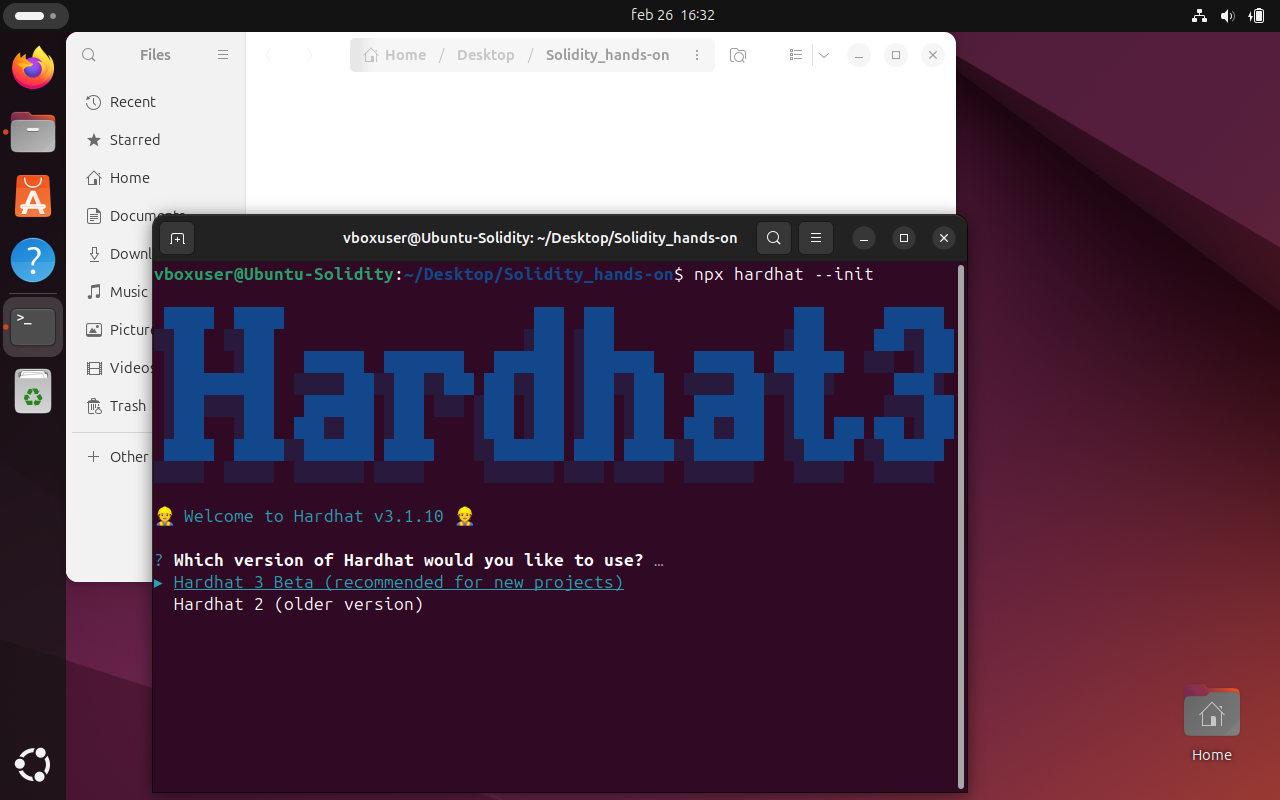
\includegraphics[width=\linewidth]{Images/Hardhat init.png}
    \caption{Hardhat initialization}
    \label{fig:hardhat_init}
\end{figure}

\section{Anatomy of a Hardhat Project}

The initialization process creates several key directories and files, each with a distinct purpose:

\begin{itemize}
    \item
    \texttt{contracts:} This folder is the designated location for all Solidity smart contract source files (files with a \texttt{.sol} extension). This is where the core logic of your application will reside.

    \item
    \texttt{ignition:} This folder contains TypeScript scripts that leverage the \textbf{Hardhat Ignition} module. These scripts define the deployment logic for your smart contracts in a declarative way, ensuring that the process of deploying to any network is simple and reliable.

    \item
    \texttt{node\_modules:} It is the folder containing all project dependencies — that is, the libraries and packages you have installed (Hardhat, ethers.js, Mocha, TypeScript, etc.). It is generated automatically when you run \texttt{npm install}. It is very large (contains thousands of files) and should never be committed to Git (it is usually in \texttt{.gitignore}).
    
    \item
    \texttt{test:} This directory holds your validation logic. It supports two distinct testing philosophies: fast, internal unit tests written in Solidity (often ending in \texttt{.t.sol}) that execute directly within the EVM, and external integration tests written in TypeScript/JavaScript that interact with the contract from the outside, simulating how a front-end or other service would.
    
    \item
    \texttt{hardhat.config.js} (or \texttt{.ts}) This is the central configuration file for the project. It is where you define network details, such as connections to a local simulated node, public testnets like Sepolia, or the production Ethereum mainnet. It also configures the Solidity compiler version and other project-wide settings.

    \item
    \texttt{package.json:} It is the main configuration file of your project. It contains important metadata such as the project name, version, required dependencies (both direct and development), and npm scripts you can run. When you share the project with others, they will have this file and can recreate the entire environment by running \texttt{npm install}.

    \item
    \texttt{package-lock.json:} It is a file automatically generated by npm that ''freezes'' the exact versions of all installed dependencies (including sub-dependencies). It ensures that anyone who clones the project obtains exactly the same versions, avoiding incompatibilities. It is important to commit it to Git along with \texttt{package.json}.

    \item
    \texttt{README.md:} It is a documentation file in Markdown format that describes your project: what it does, how to install it, how to use it, etc. It is the first file others read when they see your repository. Hardhat generates a base template that you can customize.

    \item
    \texttt{tsconfig.json:} It is the TypeScript configuration file. It specifies how the TypeScript compiler should behave: which JavaScript version to target, which modules to use, where to look for source files, etc. It allows TypeScript to correctly convert your \texttt{.ts} code into executable JavaScript.
\end{itemize}

With the project structure in place, we can now focus on the specific smart contract we will be building.

\chapter{Dissecting the Purchase.sol Smart Contract}

The example contract we will build, \texttt{Purchase.sol}, implements a ''Safe Remote Purchase'' pattern. This is a common and practical use case for smart contracts, where an agreement is enforced by code to create trust between a buyer and a seller without relying on a traditional third-party intermediary. The contract acts as a digital escrow, holding funds until specific conditions are met by both parties. \\

To proceed with the hands-on lesson go to the "contracts" folder, create a file, call it "Purchase.sol", copy the code from the "\href{https://docs.soliditylang.org/en/latest/solidity-by-example.html#safe-remote-purchase}{Safe Remote Purchase}" section of the official Solidity website and paste it in the newly created file.

\section{Core Logic and State Machine}

The contract's core function is to manage an escrow process. To initiate a sale, a seller deploys the contract and deposits funds equal to \textbf{twice the item's value}. To proceed, a buyer must also deposit funds equal to \textbf{twice the item's value}. These funds remain locked within the contract until the buyer explicitly confirms they have received the item. This mechanism ensures both parties have significant ''skin in the game'', incentivizing them to complete the transaction honestly.\\

The contract's logic is governed by a simple state machine defined by the \texttt{State} enum:

\begin{enumerate}
    \item
    \texttt{Created}: The initial state after the seller deploys the contract and deposits their escrow. The contract is awaiting a buyer.
    
    \item
    \texttt{Locked}: The state after a buyer has called \texttt{confirmPurchase()} and deposited their corresponding escrow. Both parties' funds are now locked.
    
    \item
    \texttt{Release}: The state after the buyer has called \texttt{confirmReceived()}, signaling the item has been delivered. Funds are now ready for distribution.
    
    \item
    \texttt{Inactive}: The final state after the transaction is successfully completed and all funds have been paid out, or after the transaction has been aborted.
\end{enumerate}

\section{Key Functions and Modifiers}

The contract's behavior is exposed through several public functions, with access controlled by modifiers that restrict who can call them and in what state.\\

\begin{tabularx}{\linewidth}{|>{\raggedright\arraybackslash}l|>{\raggedright\arraybackslash}l|>{\raggedright\arraybackslash}X|}
    \hline
    
    \textbf{Function/Modifier} & \textbf{Role} & \textbf{Action} \\
    \hline
    
    \texttt{constructor()} & Seller & Deploys the contract, sets the item's \texttt{value}, and locks the seller's initial deposit (which is 2x the \texttt{value}). \\
    \hline
    
    \texttt{onlySeller}/\texttt{onlyBuyer} & System & These modifiers restrict function execution, ensuring that only the designated seller or buyer can perform certain critical actions. \\
    \hline
    
    \texttt{confirmPurchase()} & Buyer & Deposits funds equal to \texttt{2 * value} to lock in the purchase and transitions the contract's state to \texttt{Locked}. \\
    \hline
    
    \texttt{confirmReceived()} & Buyer & Confirms the item was delivered, transitions the state to \texttt{Release}, and triggers a refund of \texttt{value} (half of the buyer's total deposit) back to the buyer. \\
    \hline
    
    \texttt{refundSeller()} & Seller & Called after the buyer's confirmation. It pays the seller \texttt{3 * value} (their original \texttt{2 * value} deposit plus the \texttt{value} of the item) and sets the state to \texttt{Inactive}. \\
    \hline
    
    \texttt{abort()} & Seller & Can only be called in the \texttt{Created} state. This cancels the sale, refunds the seller's full deposit, and sets the state to \texttt{Inactive}. \\
    \hline
\end{tabularx}
\vspace{1em}

\section{Clarifications about the code}

In the body of the modifiers we can see the following command: \texttt{"\_;"}. This is a placeholder for the body of the functions to which the modifier will be applied. This means that modifiers can be used as preconditions or post-conditions to the other functions depending on the cases. This makes Solidity more flexible and less error prone.\\

In the body of the constructor we can see that the value of the item is set as the half of the message value and then the code checks if the message value is an even number by checking that the double of the item value is equal to the message value. This process may seem unnecessary but it follows naturally from the need to first compute the item value and then verify that no precision was lost in the integer division, making the check a logical consequence of the assignment rather than an independent precondition. Basically, if the message value was an odd number the result of the division by 2 would have been the floor approximation of the actual result and doubling the item value wouldn't have led to finding the message value.\\
One could have also checked the parity of the message value before performing the division using a modulo operator (\texttt{msg.value \% 2 == 0}) or the bitwise \texttt{\&} for higher performances (\texttt{msg.value \& 1 == 0}) and would have achieved the same result.\\

Now that we understand the contract's code, we can move on to the practical steps of compiling, testing, and deploying it.

\chapter{The Core Workflow: Compiling, Testing, and Deploying}

The smart contract development lifecycle follows an essential, sequential path. Once the Solidity code is written, it must be compiled into Ethereum Virtual Machine (EVM) bytecode, rigorously tested to identify and eliminate bugs, and finally deployed to a network to become operational. Hardhat streamlines each of these critical stages with simple command-line instructions.

\section{Compilation and Testing}

First, the entire project, including all contracts and their dependencies, can be compiled with a single command:

\begin{lstlisting}
    npx hardhat compile
\end{lstlisting}

After a successful compilation, you can run all associated tests using:

\begin{lstlisting}
    npx hardhat test
\end{lstlisting}

This command automatically discovers and executes all test files within the \texttt{test/} directory, running both Solidity-based unit tests and TypeScript-based integration tests. This unified test runner is a cornerstone of the Hardhat workflow, ensuring that both high-level behavior and low-level contract logic are validated before any deployment is considered. Never deploy untested code.\\

How to write tests is not part of the syllabus of this course but you can generate a TypeScript tests file using AI, put it in the \texttt{test} folder and run the tests using the aforementioned command. You will see an output similar to the one depicted in figure ~\ref{fig:npx_hardhat_test}.

\begin{figure}
    \centering
    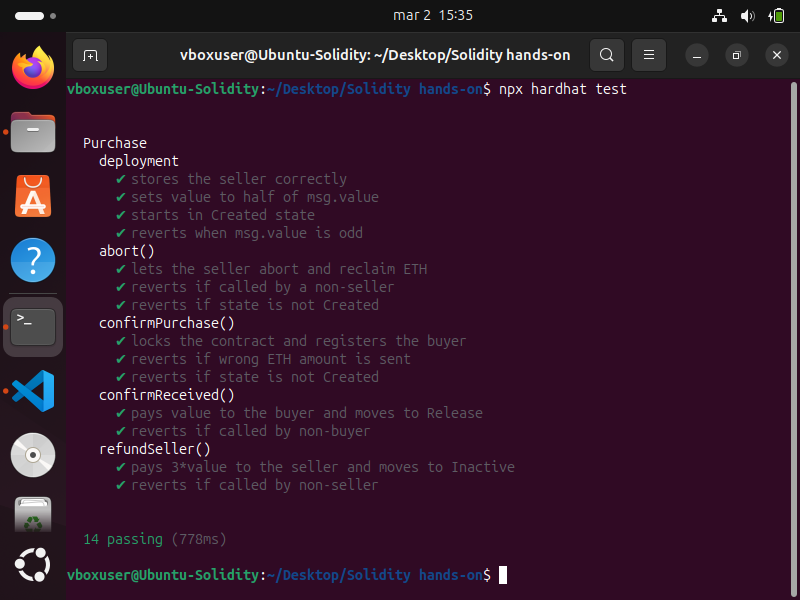
\includegraphics[width=\linewidth]{Images/npx hardhat test.png}
    \caption{Running tests automatically in Hardhat}
    \label{fig:npx_hardhat_test}
\end{figure}

\section{Running a Local Network}

For rapid development and testing, Hardhat allows you to run a simulated Ethereum network directly on your local machine. To start this network, use the command:

\begin{lstlisting}
    npx hardhat node
\end{lstlisting}

This local node provides a complete, sandboxed blockchain environment that includes:

\begin{itemize}
    \item A JSON-RPC server that perfectly mimics a real Ethereum network, allowing tools like MetaMask to connect to it.
    
    \item A set of pre-generated, externally owned test accounts.
    
    \item A starting balance of 10,000 ''fake'' ETH for each test account, which can be used to pay for gas fees during development and testing without any real-world cost.
\end{itemize}

\section{Deploying the Contract}

With a local network running, the next step is to deploy the smart contract. This process is managed by the scripts located in the \texttt{ignition/} folder. To execute a deployment script, you specify the script's path and the target network:

\begin{lstlisting}
    npx hardhat ignition deploy \
    ignition/modules/Purchase.ts --network localhost
\end{lstlisting}

How to create an ignition deployment script is not part of the syllabus of this course but you can generate it using AI, call it \texttt{Purchase.ts} and put it in the \texttt{ignition/modules} folder.\\

A successful deployment will output the address of the newly created smart contract on the local blockchain. This address is the unique identifier for your contract instance and is essential for the final phase: interaction.\\

With the contract compiled, tested, and deployed, it is now live on our local network and ready to be interacted with.

\chapter{Interacting with the Deployed Contract via Remix}

While command-line tools are powerful, a graphical user interface (GUI) can provide a more intuitive way to interact with a deployed contract and verify its functionality. The Remix IDE, an online Solidity development environment, is an excellent tool for this purpose. We can connect it to our local Hardhat node to call contract functions and observe state changes in real-time.

\section{Connecting Remix to the Local Hardhat Node}

This process effectively uses Remix as a powerful GUI to ''attach'' to a contract managed by our terminal-based Hardhat environment, a common pattern for quick, visual interaction without leaving your primary workflow.\\

There are two equivalent ways to connect Remix IDE to our local Hardhat environment: using an injected provider like MetaMask or by using an external HTTP provider.

\subsection{Using MetaMask as an injected provider}

Before we begin with the procedure note that some versions of MetaMask do not allow us to use MetaMask as an intermediary between our local Hardhat environment and the Remix IDE. If that's the case, it won't be possible to run transactions through MetaMask but we can still use the latter to monitor the balances of the accounts we use for the transactions using the other method.

\begin{enumerate}
    \item Set up MetaMask and connect it to the local hardhat network following this guide: \href{https://medium.com/@kaishinaw/connecting-metamask-with-a-local-hardhat-network-7d8cea604dc6}{Connecting MetaMask with a Local Hardhat Network}.

    \item Select an imported account (see figure ~\ref{fig:select_an_imported_account_in_metamask}).

    \item Keep the MetaMask tab open in the browser and open a new tab.
    
    \item In the ``Environment'' dropdown, change the selection from ``Remix VM'' to an ``Injected Provider'' (like MetaMask). Your MetaMask wallet should be configured to connect to your local Hardhat network (e.g., \texttt{localhost:8545}) if you followed the guide correctly.
    After you select this dropdown option you will see the inteface depicted in figure ~\ref{fig:injected_provider_selection}. The account you see in the interface is the one you selected in the MetaMask tab of your browser.
    
    \item At this point you can see the selected account in the "ACCOUNT" dropdown menu and, if the balance of the account is 0 Ether, it means that the current version of MetaMask does not support this operation (see figure ~\ref{fig:balance_of_0_ether}). 
\end{enumerate}

\begin{figure}
    \centering
    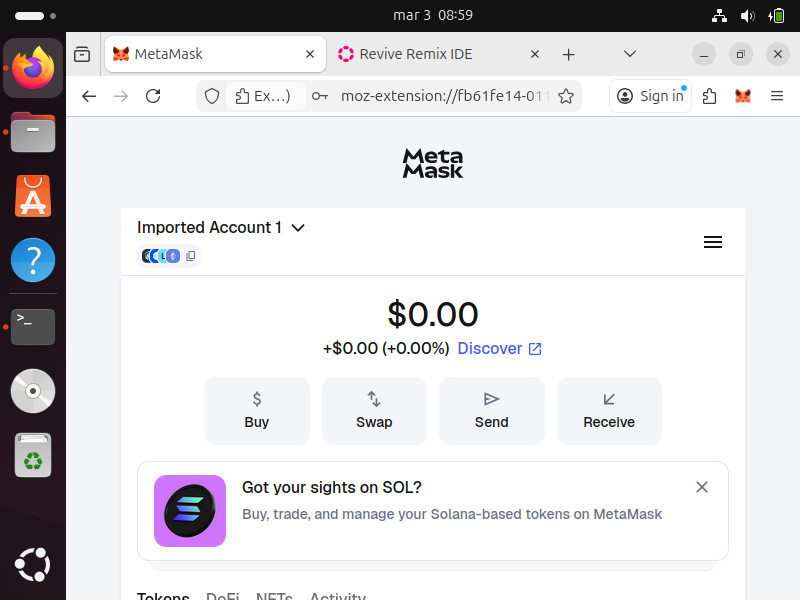
\includegraphics[width=0.5\linewidth]{Images/Select an imported account in MetaMask.png}
    \caption{Select an imported account in MetaMask}
    \label{fig:select_an_imported_account_in_metamask}
\end{figure}

\begin{figure}
    \centering
    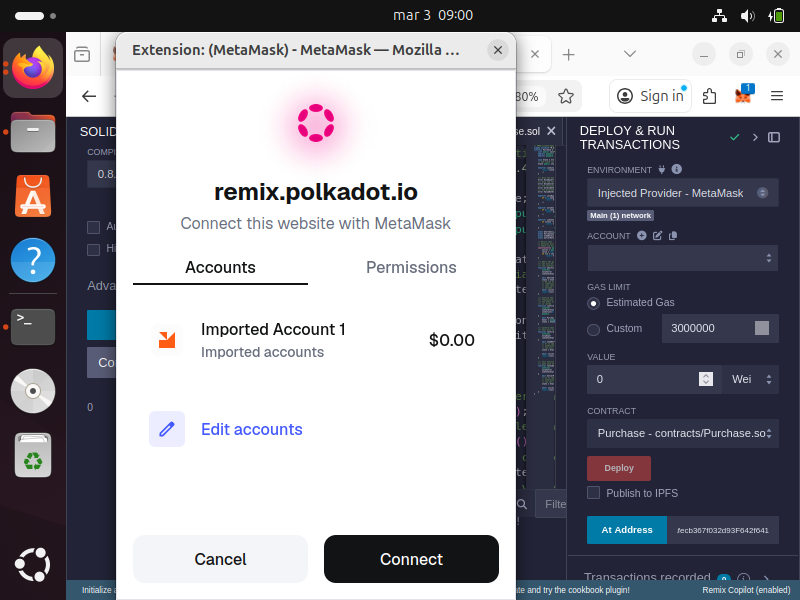
\includegraphics[width=0.5\linewidth]{Images/Injected provider selection.png}
    \caption{Injected provider selection}
    \label{fig:injected_provider_selection}
\end{figure}

\begin{figure}
    \centering
    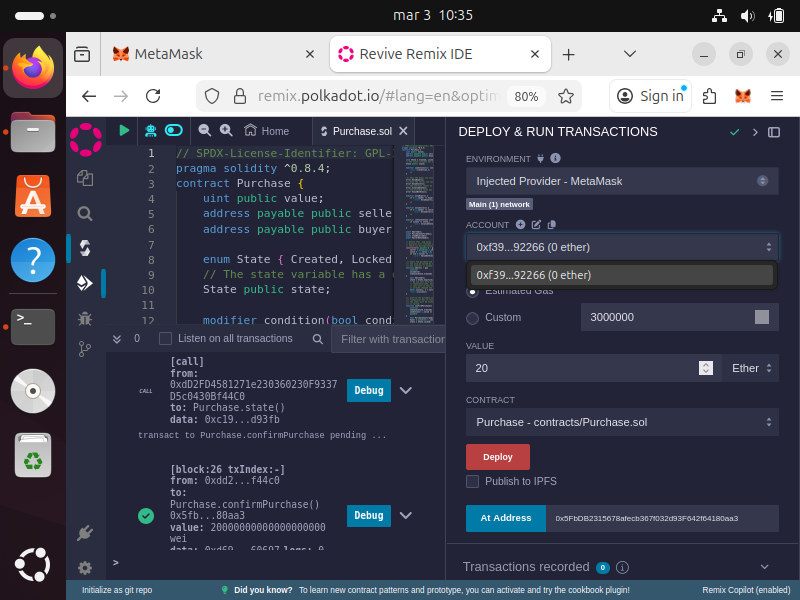
\includegraphics[width=0.5\linewidth]{Images/Balance of 0 Ether.png}
    \caption{The account has a balance of 0 Ether because the current version of MetaMask does not support the procedure}
    \label{fig:balance_of_0_ether}
\end{figure}

\subsection{Using an external HTTP provider}

Using an external HTTP provider directly connects the Remix IDE to our local Hardhat environment. 

\begin{enumerate}
    \item In the Remix IDE go to the ``Deploy \& Run Transactions'' tab on the sidebar on the left, click the "ENVIRONMENT" dropdown menu and select "Customize this list...".

    \item In the menu, search for the option that says "Deploy to a custom local network" and tick the mark in the top-right corner of the box (see figure ~\ref{fig:adding_an_environment}).

    \item Now we should be able to see and select the "Custom - External Http Provider" option in the environment dropdown.

    \item When the popup in figure ~\ref{fig:external_http_provider_popup} shows up, press Enter.

    \item Now, in the account dropdown we should be able to select one of the many accounts we have created using the \texttt{npx hardhat node} command and select one (see figure ~\ref{fig:local_hardhat_accounts_list}).
\end{enumerate}

\begin{figure}
    \centering
    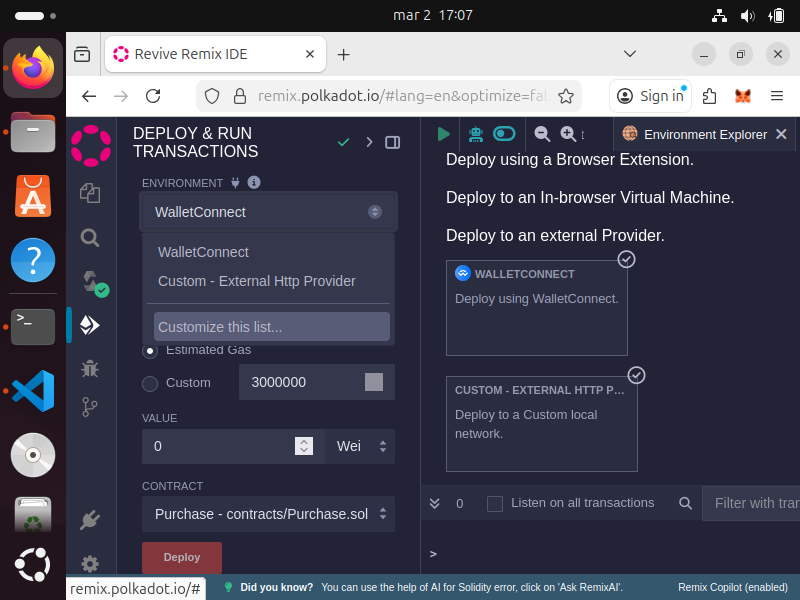
\includegraphics[width=0.5\linewidth]{Images/Remix environment addition.png}
    \caption{Adding an environment in Remix IDE}
    \label{fig:adding_an_environment}
\end{figure}

\begin{figure}
    \centering
    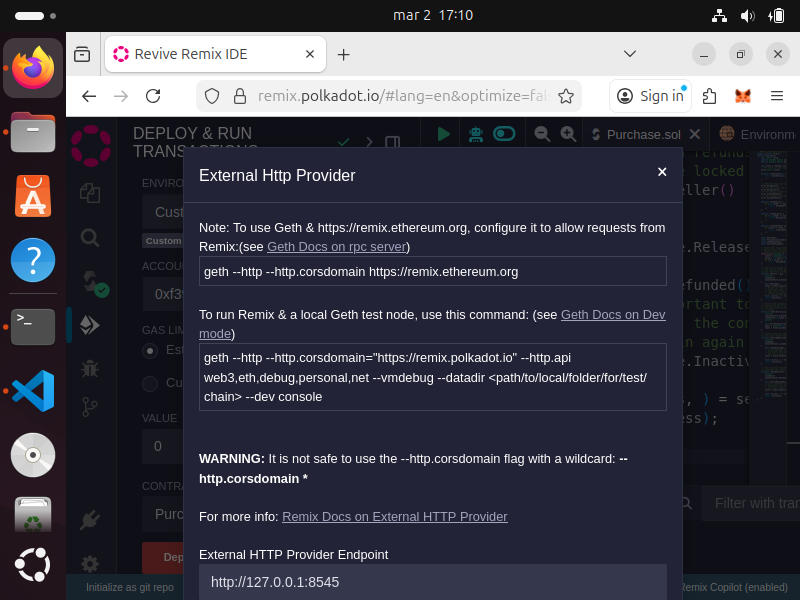
\includegraphics[width=0.5\linewidth]{Images/External HTTP provider menu.png}
    \caption{External HTTP provider popup}
    \label{fig:external_http_provider_popup}
\end{figure}

\begin{figure}
    \centering
    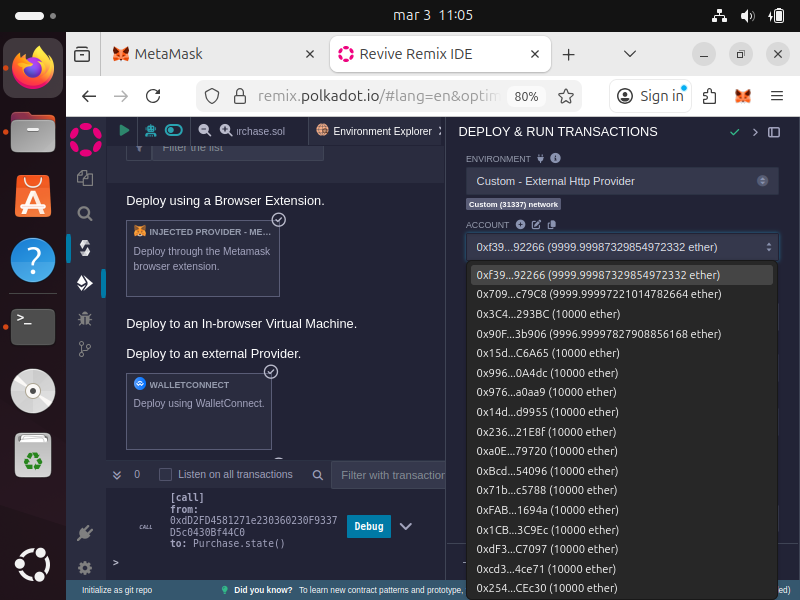
\includegraphics[width=0.5\linewidth]{Images/Local hardhat accounts list.png}
    \caption{Local Hardhat accounts list}
    \label{fig:local_hardhat_accounts_list}
\end{figure}

\subsection{Compiling and deploying the contract}

\begin{enumerate}
    \item Go to the Remix IDE, create a new file (e.g., \texttt{Purchase.sol}) and paste the exact source code of your smart contract into it.
    
    \item Compile the contract within Remix. This step does not deploy a new instance; instead, it provides Remix with the contract's Application Binary Interface (ABI), which is the ``manual'' for how to interact with its functions.
    
    \item Navigate to the ``Deploy \& Run Transactions'' tab on the sidebar on the left in Remix.

    \item Instead of using the ``Deploy'' button, find the ``At Address'' field. Paste the contract address you obtained from the Hardhat deployment step (see figure ~\ref{fig:contract_address_generated_during_deployment}) into this field and click the button at its side (see figure ~\ref{fig:insertion_of_the_contract_address}).
\end{enumerate}

\begin{figure}
    \centering
    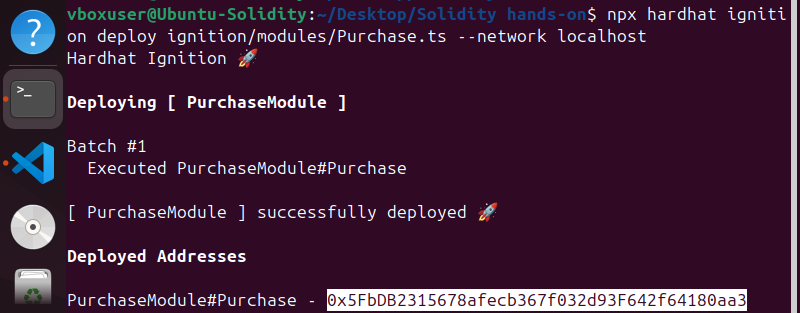
\includegraphics[width=0.5\linewidth]{Images/Contract address.png}
    \caption{Contract address generated during the deployment phase}
    \label{fig:contract_address_generated_during_deployment}
\end{figure}

\begin{figure}
    \centering
    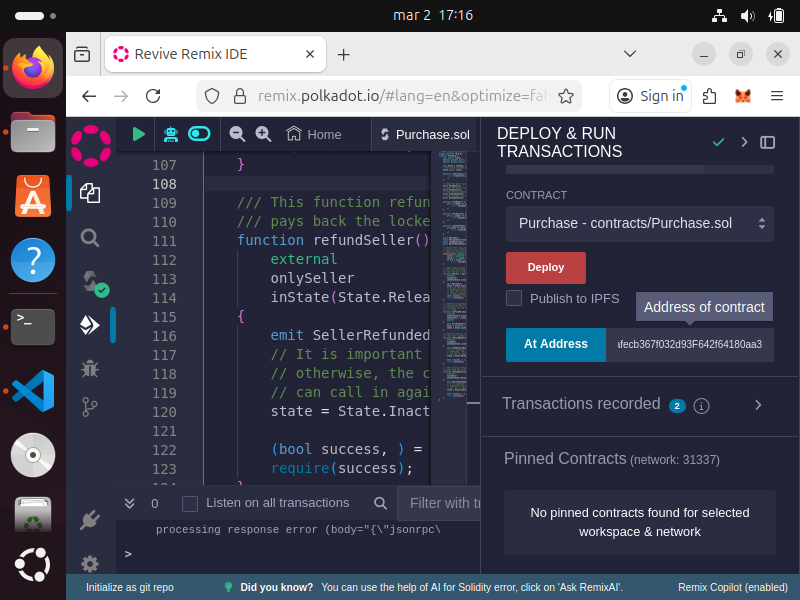
\includegraphics[width=0.5\linewidth]{Images/Paste the contract address.png}
    \caption{Insertion of the contract address}
    \label{fig:insertion_of_the_contract_address}
\end{figure}

\section{Calling Contract Functions}

After successfully connecting Remix to the contract address, navigate to the bottom of the column and click the arrow at the left end of the deployed contract (see figure ~\ref{fig:deployed_contract}). The IDE will display a user interface with clickable buttons for all the public functions of the \texttt{Purchase} contract (see figure ~\ref{fig:deployed_contract_functions}).\\

You can now call functions on the contract using the buttons on the interface. For \texttt{payable} functions like \texttt{confirmPurchase}, you must also specify the amount of Ether you wish to send with the transaction in the input field right above the contract field (see figure ~\ref{fig:enter_the_transaction_value}). After calling a function, we can see its results in the Remix IDE terminal in the bottom-left end of the screen (see figure ~\ref{fig:transaction_result_remix_ide}) and in the Hardhat node console on our local machine (see figure ~\ref{fig:transaction_result_hardhat_node}).\\

Now that we issued the transaction, we can see that the value of the transaction was deducted from the account using both the Remix IDE (see figure ~\ref{fig:new_balance_remix_IDE}) and MetaMask (see figure ~\ref{fig:new_balance_metamask}).\\

This end-to-end process allows for complete validation of the contract's logic and behavior in a controlled, interactive environment.

\begin{figure}
    \centering
    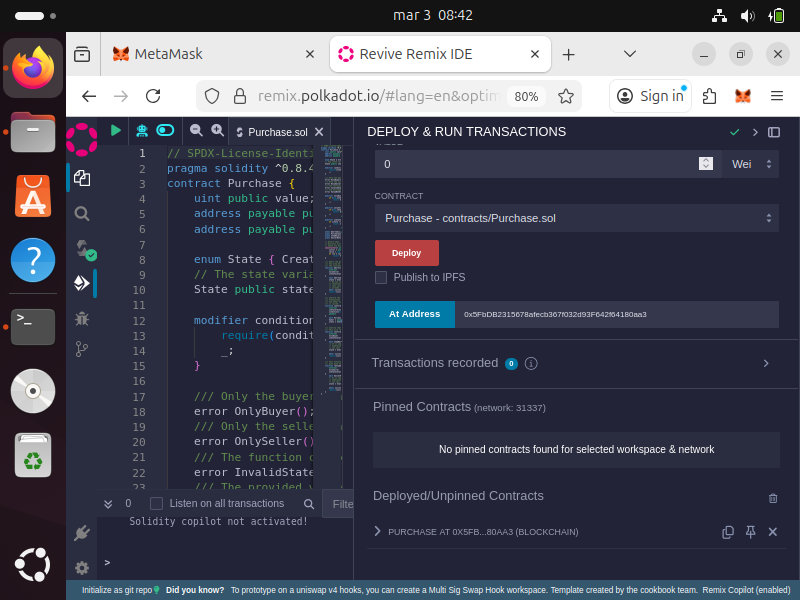
\includegraphics[width=0.5\linewidth]{Images/Deployed contract.png}
    \caption{Deployed contract}
    \label{fig:deployed_contract}
\end{figure}

\begin{figure}
    \centering
    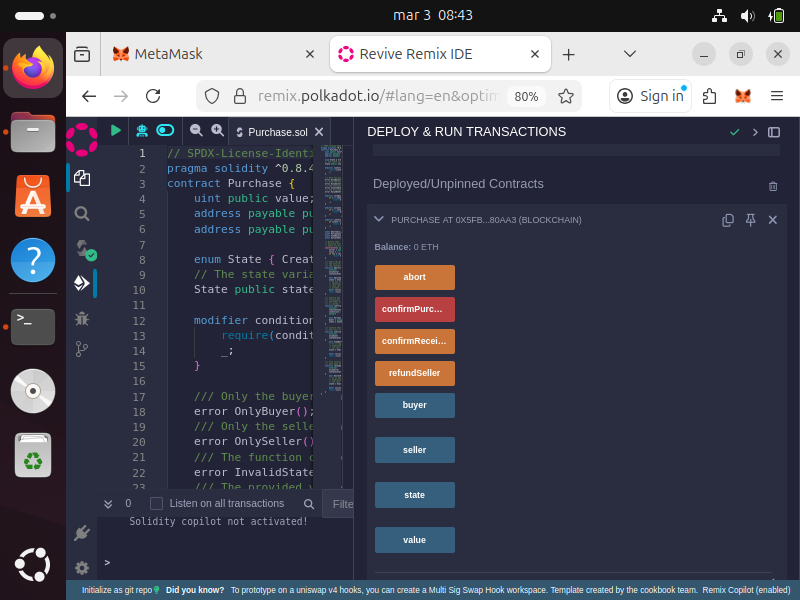
\includegraphics[width=0.5\linewidth]{Images/Deployed contract functions.png}
    \caption{Deployed contract functions}
    \label{fig:deployed_contract_functions}
\end{figure}

\begin{figure}
    \centering
    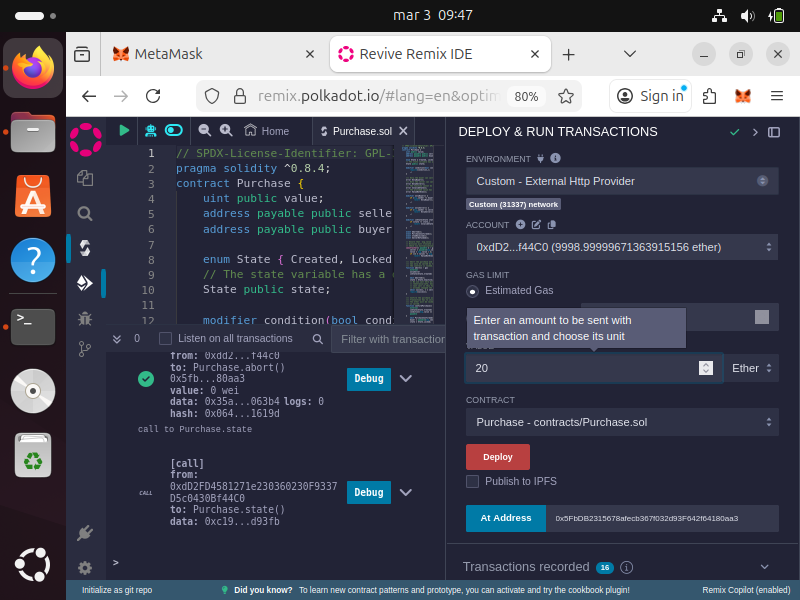
\includegraphics[width=0.5\linewidth]{Images/Enter the transaction value.png}
    \caption{Enter the transaction value}
    \label{fig:enter_the_transaction_value}
\end{figure}

\begin{figure}
    \centering
    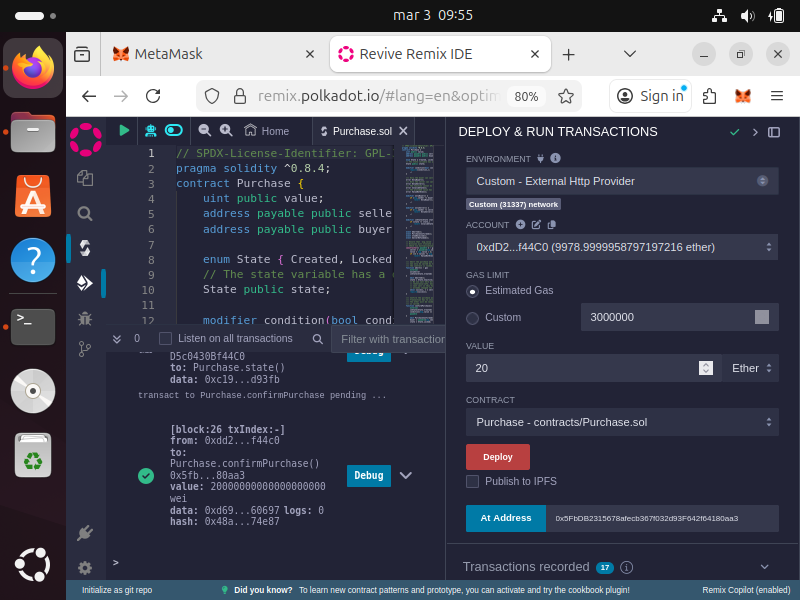
\includegraphics[width=0.5\linewidth]{Images/Transaction result Remix IDE.png}
    \caption{Transaction result in the Remix IDE - Notice that the value of 20 Ether was converted in Wei}
    \label{fig:transaction_result_remix_ide}
\end{figure}

\begin{figure}
    \centering
    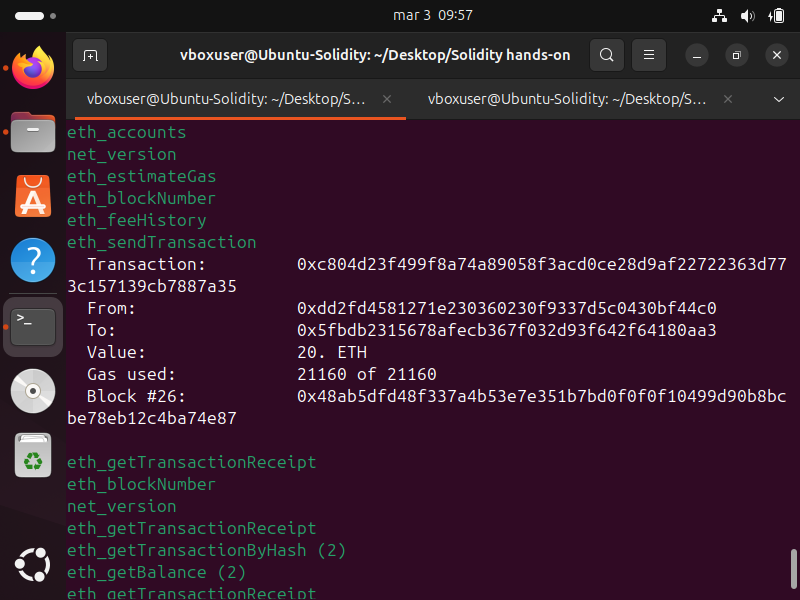
\includegraphics[width=0.5\linewidth]{Images/Transaction result local machine.png}
    \caption{Transaction result in the Hardhat node console on our local machine}
    \label{fig:transaction_result_hardhat_node}
\end{figure}

\begin{figure}
    \centering
    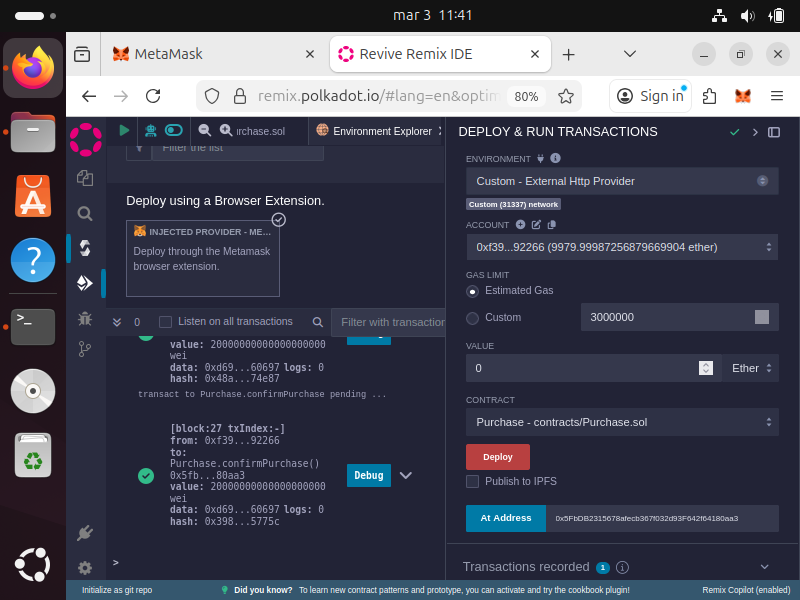
\includegraphics[width=0.5\linewidth]{Images/New balance remix ide.png}
    \caption{New balance of the account in the Remix IDE}
    \label{fig:new_balance_remix_IDE}
\end{figure}

\begin{figure}
    \centering
    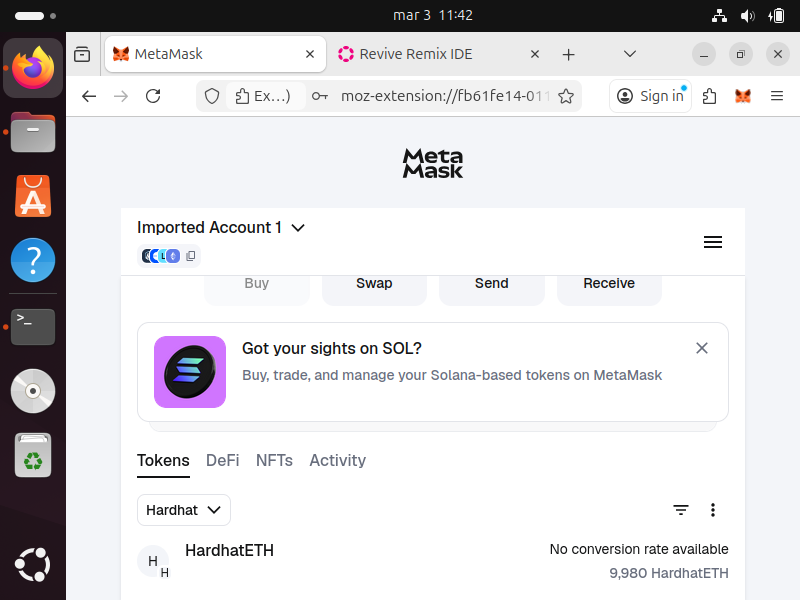
\includegraphics[width=0.5\linewidth]{Images/New balance metamask.png}
    \caption{New balance of the account in MetaMask - In this case the number is rounded}
    \label{fig:new_balance_metamask}
\end{figure}

\chapter{Conclusion}

This guide has walked through the complete, end-to-end workflow of modern smart contract development. We covered setting up a professional development environment with Hardhat, organizing a project with its logical structure, writing a stateful Solidity contract for a real-world use case, and then systematically compiling, testing, deploying, and interacting with it. By leveraging industry-standard tools like Hardhat for the backend lifecycle and MetaMask and Remix for frontend interaction, developers can build, validate, and deploy robust decentralized applications with confidence. Mastering this workflow is a fundamental competency for any developer looking to build on the blockchain.

\end{document}
